\documentclass[t]{beamer}

\mode<presentation>
{
  \usetheme{default}
  \setbeamertemplate{navigation symbols}{}
  \setbeamertemplate{footline}[frame number]
  \setbeamertemplate{items}[circle]
  \usecolortheme{seahorse}
}

\usepackage[english]{babel}
\usepackage[utf8]{inputenc}
\usepackage{times}
\usepackage[T1]{fontenc}
\usepackage{url}
\usepackage{amsmath}

\parskip=8 pt

\newcommand\topstrut{\rule{0pt}{2.6ex}}
\newcommand\bottomstrut{\rule[-1.2ex]{0pt}{0pt}}
\newcommand\doublestrut{\rule[-1.2ex]{0pt}{3.6ex}}

\newcommand\blue[1]{\textcolor{blue}{#1}}
\newcommand\red[1]{\textcolor{red}{#1}}
\newcommand\gray[1]{\textcolor{gray}{#1}}
\newcommand\smallgray[1]{\textcolor{gray}{\small\it #1}}
\newcommand\prevwork[1]{\smallgray{#1}}

\title
{Statistics for Machine Learning and Big Data}
\subtitle{An Introduction}

\author[Abrahamson] {Jeff Abrahamson}

% If you wish to uncover everything in a step-wise fashion, uncomment
% the following command: 
%\beamerdefaultoverlayspecification{<+->}

\begin{document}

\begin{frame}
  \titlepage
\end{frame}

\begin{frame}
  \frametitle{Useful facts}

  \only<1>{\centerline{I am a computer scientist.}}
  \only<2>{\centerline{Python is a useful tool.}}

  \note{
    My goal is to understand computer science and machine learning.

    Our goal this week is to understand statistics and to use python
    to help us.  Not to learn anything in particular about python.
  }
\end{frame}

\section{Probability}

\begin{frame}
  \frametitle{Review}
  \begin{itemize}
  \item Counting
  \item Urns (sampling)
  \item Area
  \end{itemize}
\end{frame}

\begin{frame}
  \frametitle{}

\end{frame}

\begin{frame}
  \frametitle{Counting}

  Example: two children, what is $P(\exists \mathrm{boy}) = P(\exists b)$?

  \only<2>{graphic of bb, bg, gb, gg with prob 1/4}
  \only<3->{graphic of bb, bg, gb, gg with prob 1/4 with circled if $\exists$ b}
  \only<4->{What about $P(\exists b \mid \exists g)$?}
  \only<5->{same graphic, fade bb, circles, show 2/3}
  \only<6->{Events have probabilities summing to 1, cover, and are disjoint.}
\end{frame}

\begin{frame}
  \frametitle{Pólya urn model}

  $r$ red balls, $b$ black balls in an urn.

  \only<2->{
  \begin{itemize}
  \item Sampling with replacement and duplication (rich get richer)
  \item Variations: balls into boxes
    \begin{itemize}
    \item Sampling with replacement
    \item Sampling without replacement
    \end{itemize}
  \end{itemize}
  }
  \only<3->{Want to know sequence of colours selected, evolution of colour distribution in urn.}
\end{frame}

\begin{frame}
  \frametitle{Sampling}

  \begin{itemize}
  \item We don't know $r$, $b$, or even $r/b$.  Estimate.
  \end{itemize}

  % http://en.wikipedia.org/wiki/Simple_random_sample
  % http://en.wikipedia.org/wiki/Urn_problem
\end{frame}

\begin{frame}
  \frametitle{Area}

  \begin{itemize}
  \item Continuous case.
  \item Events are regions.
  \item Same constraints: sum of areas is unity.  Cover and disjoint.
  \item Zero probability events!
  \end{itemize}
\end{frame}

\begin{frame}
  \frametitle{Distributions}

  Sneak preview of some common distributions, what they look like, and processes giving rise to them.
\end{frame}


\section{Statistics}
%\subsection{Subsection}

\begin{frame}
  \frametitle{What is statistics?}
  \begin{enumerate}
  \item<1-> Identify a question or problem.
  \item<1-> Collect relevant data on the topic.
  \item<1-> Analyze the data.
  \item<1-> Form a conclusion.
  \end{enumerate}
  \only<2>{Sadly, sometimes people forget 1.}
  \only<3->{Statistics is about making 2--4 efficient, rigorous, and meaningful.}
  \only<4>{\prevwork{\textit{OpenIntro Statistics}, 2nd edition, D.~Diez, C.~Barr, M.~Çetinkaya-Rundel, 2013.}}
\end{frame}


\begin{frame}
  \frametitle{Significance}

  \begin{itemize}
  \item Flip a coin $N$ times.  Get 49\% heads.  Is the coin fair?
  \item Congress/parliament has $N$ members of whom $m$ are male.  Do
    we discriminate against women?
  \item Do we discriminate against women more or less than we
    discriminate against blacks?
  \item Email classification: spam or not?
  \item Careful about what we conclude.  Here we can't conclude
    anything about cause or source.
  \end{itemize}

  % This needs supporting slides with computations.  We'll also have
  % to come back to it when we understand about $p$ values and the
  % like.
  
\end{frame}

\begin{frame}
  \frametitle{Terminology}

  \begin{itemize}
  \item A \textbf{case} or {observational unit} is an observation or a
    single sample.  E.g., an email.
  \item A \textbf{variable} is a characteristic of an observational
    unit.  E.g., number of lines, mean line length, number of words.
  \end{itemize}
  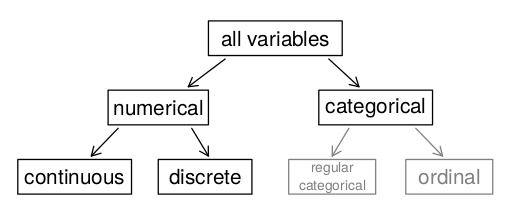
\includegraphics[width=.9\textwidth]{variable-types.png}

  Notes:  Categorical is sometimes called nominal.  Categorical
  variables with logical ordering (empty, half, full) or called ordinal.
\end{frame}

\begin{frame}
  \frametitle{Anecdote}

  Some properties of anecdote:
  
  \begin{itemize}
  \item is data
  \item haphazardly collected
  \item is generally not representative
  \item sometimes result of selective retention
  \item does not accumulate to be representative
  \item might be true (by chance)
  \item is ok to use as hypothesis, but be clear that hypothesis is anecdote
  \end{itemize}
\end{frame}

\begin{frame}
  \frametitle{Study Types}

  \begin{itemize}
  \item Observational
  \item Experimental
  \end{itemize}
  
  \note {
    
  }

  \only<2>{
    The possible gremlins:
    \begin{itemize}
    \item Association $\ne$ causation
    \item Randomness
    \item Confounding variables
    \item 
    \end{itemize}
  }
  \note {
    Example:  Sunscreen use associated with skin cancer.  But sun
    exposure is a confounding variable.

    Observational studies: prospective (identify individuals, collect
    information) and retrospective.  (Can combine the two.)
  }
\end{frame}

\begin{frame}
  \frametitle{Observational studies}

  TODO

  Can't generally conclude causation.
\end{frame}

\begin{frame}
  \frametitle{Experiment}

  We do stuff.  Maybe randomised experiment.
  
  \note{
    If well-designed, can conclude causation.

    Experiments to generate hypotheses vs experiments to demonstrate
    hypotheses.  (Don't use the same data!)

    Example: Phase 0 (10 people) and phase 1 (20-100 people) clinical trials are not randomised.

    Phase 0:  Pharmacodynamics and pharmacokinetics, particularly oral
    bioavailability and half-life of the drug.  Very small,
    subtherapeutic doses.

    Phase 1:  Testing of drug on healthy volunteers for dose-ranging.
    Often subtherapeutic, but with ascending doses.  Determine whether
    a drug is safe to check for efficacy in phase 2.
  }

  \only<2>{
    \begin{itemize}
    \item Controlling
    \item Randomisation
    \item Replication
    \item Blocking \gray{(optional, advanced)}
    \end{itemize}
  }

  \only<3>{
    \begin{itemize}
    \item $H_0$: Independent (or null) hypothesis
    \item $H_A$: Alternative hypothesis
    \end{itemize}
  }

\end{frame}

\begin{frame}
  \frametitle{Simple random sampling}

  Uniform and independent.

  \note{
    \begin{itemize}
    \item Each case has the same probability of being included.
    \item Knowing that a particular case is included provides no useful information about other cases.
    \end{itemize}

    Example: Footballers in Europe, put all the names in a bucket.
  }

  \only<2>{
    The possible gremlins:
    \begin{itemize}
    \item Not actually random
    \item Convenience sample
    \item Non-response bias
    \end{itemize}
  }

\end{frame}

\begin{frame}
  \frametitle{Stratified Sampling}

  Group like with like, then usually simple random sampling of each stratum.
  
  \note{
    Divide and conquer.

    Example:  Footballers in Europe, sample $k$ from each team.
    (Hypothesis:  footballers are paid about the same within a team.)
  }

  \only<2>{
    The guaranteed gremlin: harder to analyse than simple random sampling.
  }

\end{frame}

\begin{frame}
  \frametitle{Cluster Sampling}

  Simple random sampling to form clusters, then simple random
  sampling.

  \note{
    Example:  Sample $k$ from each village.  Works if villages have high
    diversity, not so much if villages are substantially different from
    one another.

    Example:  Ebola.  SRS expensive (census of each village, then
    maybe have to visit them all).  So select $n$ villages and sample
    $k$ within each.  Hope that villages are similar enough that this
    is valid as a first step.
  }

  \only<2>{
    The guaranteed gremlin: harder to analyse than simple random sampling.
  }
\end{frame}

\begin{frame}
  \frametitle{Mean}

  \begin{itemize}
  \item Weighted and unweighted
  \item Centroid to physicists
  \end{itemize}

  \note{
    Sample mean vs true (population) mean.
  }

  \only<2-> {
    \centerline{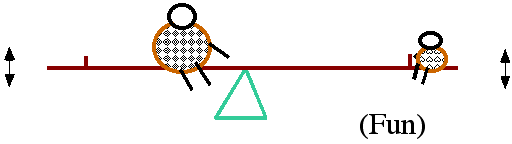
\includegraphics[width=.8\textwidth]{teeter-totter.png}}
  }
  \only<3>{
    \begin{displaymath}
      \sum w_i x_i = \mathbf{w\cdot x}
    \end{displaymath}

    \prevwork{\url{http://telescopes.stardate.org/images/research/teeter-totter/TT4.gif}}
  }
\end{frame}

\begin{frame}
  \frametitle{Variation}
  \begin{itemize}
  \item Deviation is distance from mean.
  \item Variance is mean square of deviations
  \item Standard deviation is square root of variance
  \end{itemize}
  
  \note{
    Sample standard deviation ($s$) and sample variance ($s^2$),
    divide by $n-1$.

    Population standard deviation ($\sigma$) and population variance ($\sigma^2$),
    divide by $n$.

    Population statistics may not be feasible or possible to compute.
  }

  \only<2>{
    \begin{displaymath}
      s^2 = \frac{(\overline x - x_1)^2 + \dotsb (\overline x - x_n)^2}{n-1}
    \end{displaymath}
  }
  \only<3>{
    \begin{displaymath}
      \sigma^2 = \frac{(\overline x - x_1)^2 + \dotsb (\overline x - x_MN)^2}{N}
    \end{displaymath}
  }

\end{frame}

\begin{frame}
  \frametitle{Experimental design}
  \only<1>{A telephone survey company dials digits at random (some of
    them aren't valid telephone numbers) rather than using a phone directory.
  }
  \only<2>{A statistics student wants to determine if social network
    usage among his peers (students at his school) affects academic
    performance.  Possibilities:
    \begin{itemize}
    \item He messages his class snapchat group.
    \item He posts paper fliers at his university.
    \item He gets a list of students from the registrar.  (What about
      opt-in/opt-out policies?  What if he doesn't know how many have
      opted out/failed to opt in?
    \item Other)
    \end{itemize}

  }
  \only<3>{Due to a flu epidemic, 10\% of students in a class miss the
    (final) exam.  The professor decides to offer a make-up exam but
    to require 11\% of the students who took the original exam to take
    the make-up exam as well in order to calibrate the new exam and
    make results comparable.
  }
  \only<4>{
  }
  \only<5>{
  }
  
  \note{
    Discuss.  Explain flaws.  Discuss what researcher should have done differently.
  }

\end{frame}

\begin{frame}
  \frametitle{Reasoning about data}

  \only<1>{Students at an elementary school are given a questionnaire
    that they are required to return after their parents have
    completed it. One of the questions asked is, “Do you find that
    your work schedule makes it difficult for you to spend time with
    your kids after school?” Of the parents who replied, 85\% said
    “no”. Based on these results, the school officials conclude thata
    great majority of the parents have no difficulty spending time
    with their kids after school.
  }
  \only<2>{A survey is conducted on a simple random sample of 1,000
    women who recently gave birth, asking them about whether or not they
    smoked during pregnancy. A follow-up survey asking if the children
    have respiratory problems is conducted 3 years later, however, only
    567 of these women are reached at the same address. The researcher
    reports that these 567 women are representative of all mothers.
  }
  \only<3>{An orthopedist administers a questionnaire to 30 of his
    patients who do not have any joint problems and finds that 20 of
    them regularly go running. He concludes that running decreases the
    risk of joint problems.
  }
  \only<4>{
  }
  \only<5>{
  }

  \note{
    Explain flaws.  Discuss what researcher should have done differently.
  }
  
\end{frame}

\begin{frame}
  \frametitle{Example}

  \centerline{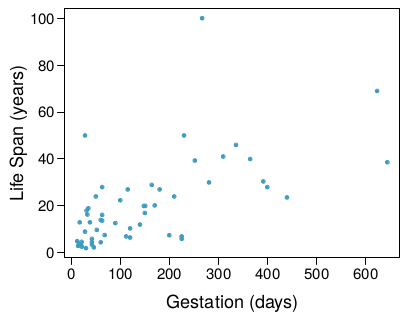
\includegraphics[width=.8\textwidth]{mammal-gestation.png}}

  \note{
    Discuss.  Are the variables independent?
  }
  
\end{frame}

\begin{frame}
  \frametitle{}

  \note{

  }
  
\end{frame}

\begin{frame}
  \frametitle{}

  \note{

  }
  
\end{frame}

\begin{frame}
  \frametitle{}

  \note{

  }
  
\end{frame}

\begin{frame}
  \frametitle{}

  \note{

  }
  
\end{frame}

\begin{frame}
  \frametitle{}

  \note{

  }
  
\end{frame}

\begin{frame}
  \frametitle{}

  \note{

  }
  
\end{frame}

\begin{frame}
  \frametitle{}

  \note{

  }
  
\end{frame}

\begin{frame}
  \frametitle{}

  \note{

  }
  
\end{frame}

\begin{frame}
  \frametitle{}

  \note{

  }
  
\end{frame}

\begin{frame}
  \frametitle{}

  \note{

  }
  
\end{frame}

\begin{frame}
  \frametitle{}

  \note{

  }
  
\end{frame}

\begin{frame}
  \frametitle{}

  \note{

  }
  
\end{frame}

\begin{frame}
  \frametitle{}

  \note{

  }
  
\end{frame}

\begin{frame}
  \frametitle{}

  \note{

  }
  
\end{frame}

\begin{frame}
  \frametitle{Questions?}
  \vspace{3cm}
  \centerline{\large\url{purple.com/talk-feedback}}
\end{frame}


\end{document}

%% ToDo:
%%
%%   Box plots
%%   Side-by-side box plots
%%   Hollow histograms
%%   Robust vs non-robust statistics (cf. log. p. 30 / phys. p. 40 in OS)
%%   Example: non-random sample before U.S. presidential, company tanked
%%     (rise of Nielson?)
%%   Example: 4 distributions with same mean, std dev
%%   
%%   Visualisation and intuition
%%   http://xkcd.com/552/
%%
%%   Tufte space shuttle data/visualisation
%%   Marathon time plots (OS, physical 70)
